\section{Motivation}\label{sec:motivation}

Private equity (PE) has experienced remarkable growth over the past two decades, emerging as a dominant force in institutional portfolios.
Global assets under management in PE exceeded USD 17 trillion in 2024 (see~\ref{fig:aum_drypowder}), with pension funds, sovereign wealth funds, and endowments allocating an increasing share of capital to the asset class.
This expansion is driven by the promise of superior returns and diversification benefits; however, PE remains fundamentally different from public markets.
Valuations are opaque, transactions are infrequent, and information is primarily controlled by general partners (GPs) through periodic reporting.
These features make it difficult to determine whether observed performance reflects true skill or risk-taking, and they place investor beliefs at the center of capital allocation decisions.

\begin{figure}[H]
    \centering
    \begin{subfigure}{0.48\textwidth}
        \centering
        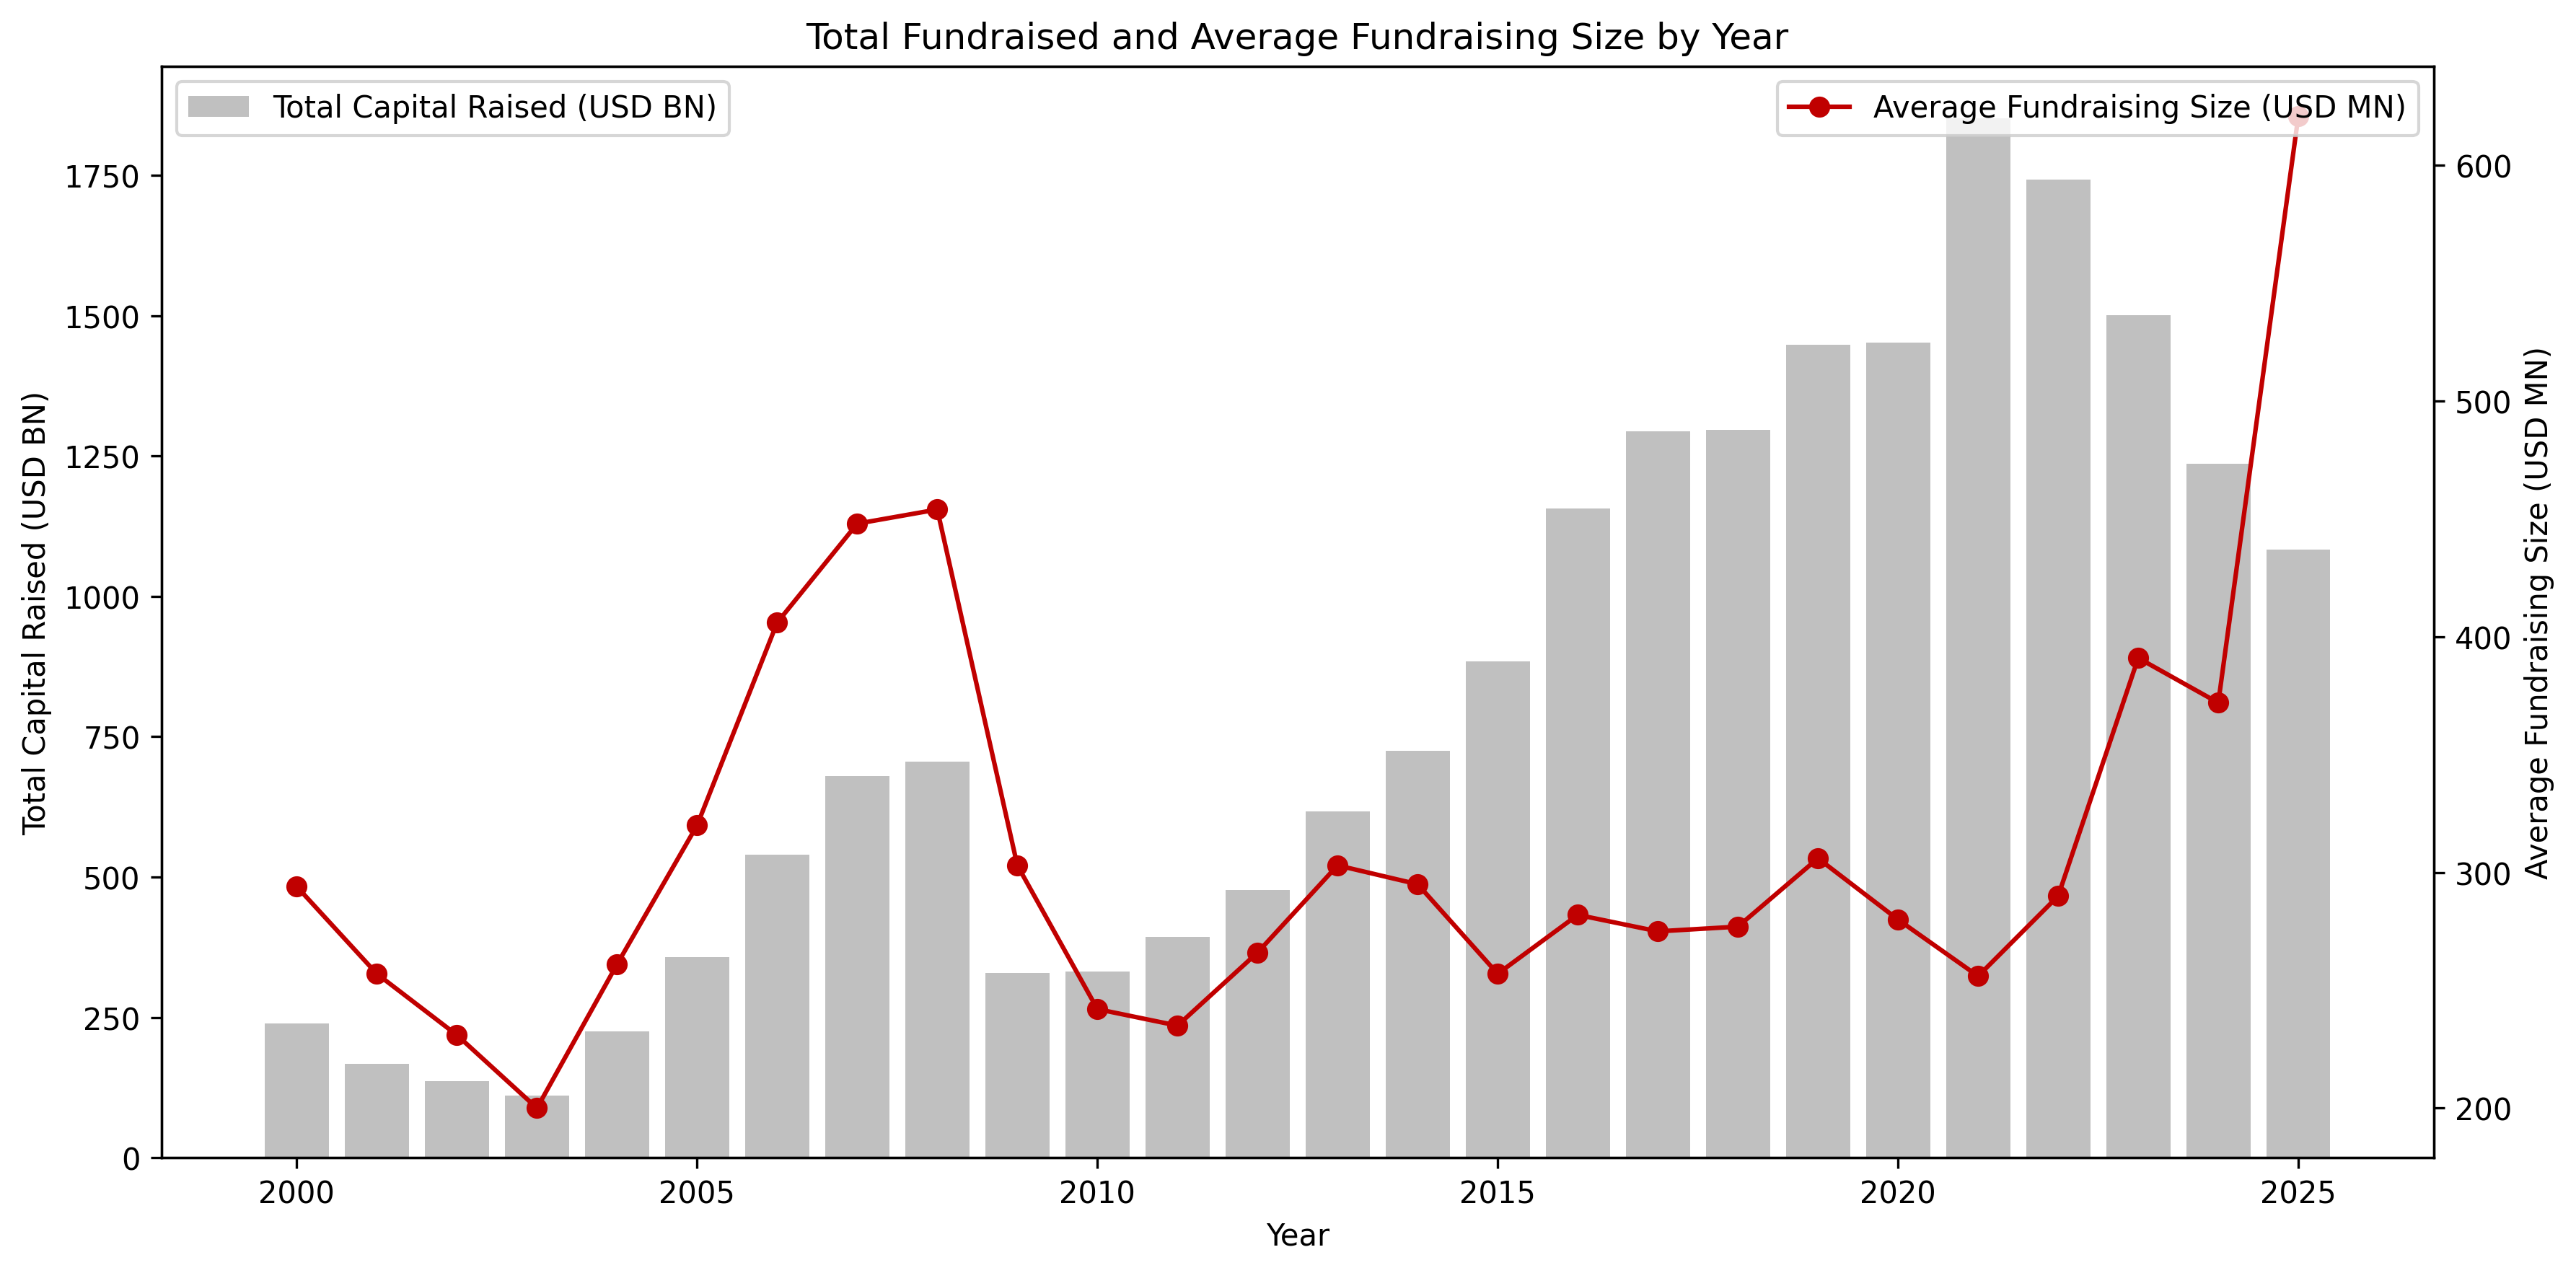
\includegraphics[width=\linewidth]{img/fundraising_vs_average}
        \caption{Private equity fundraising and average deal size.}
        \label{fig:fundraising}
    \end{subfigure}
    \hfill
    \begin{subfigure}{0.48\textwidth}
        \centering
        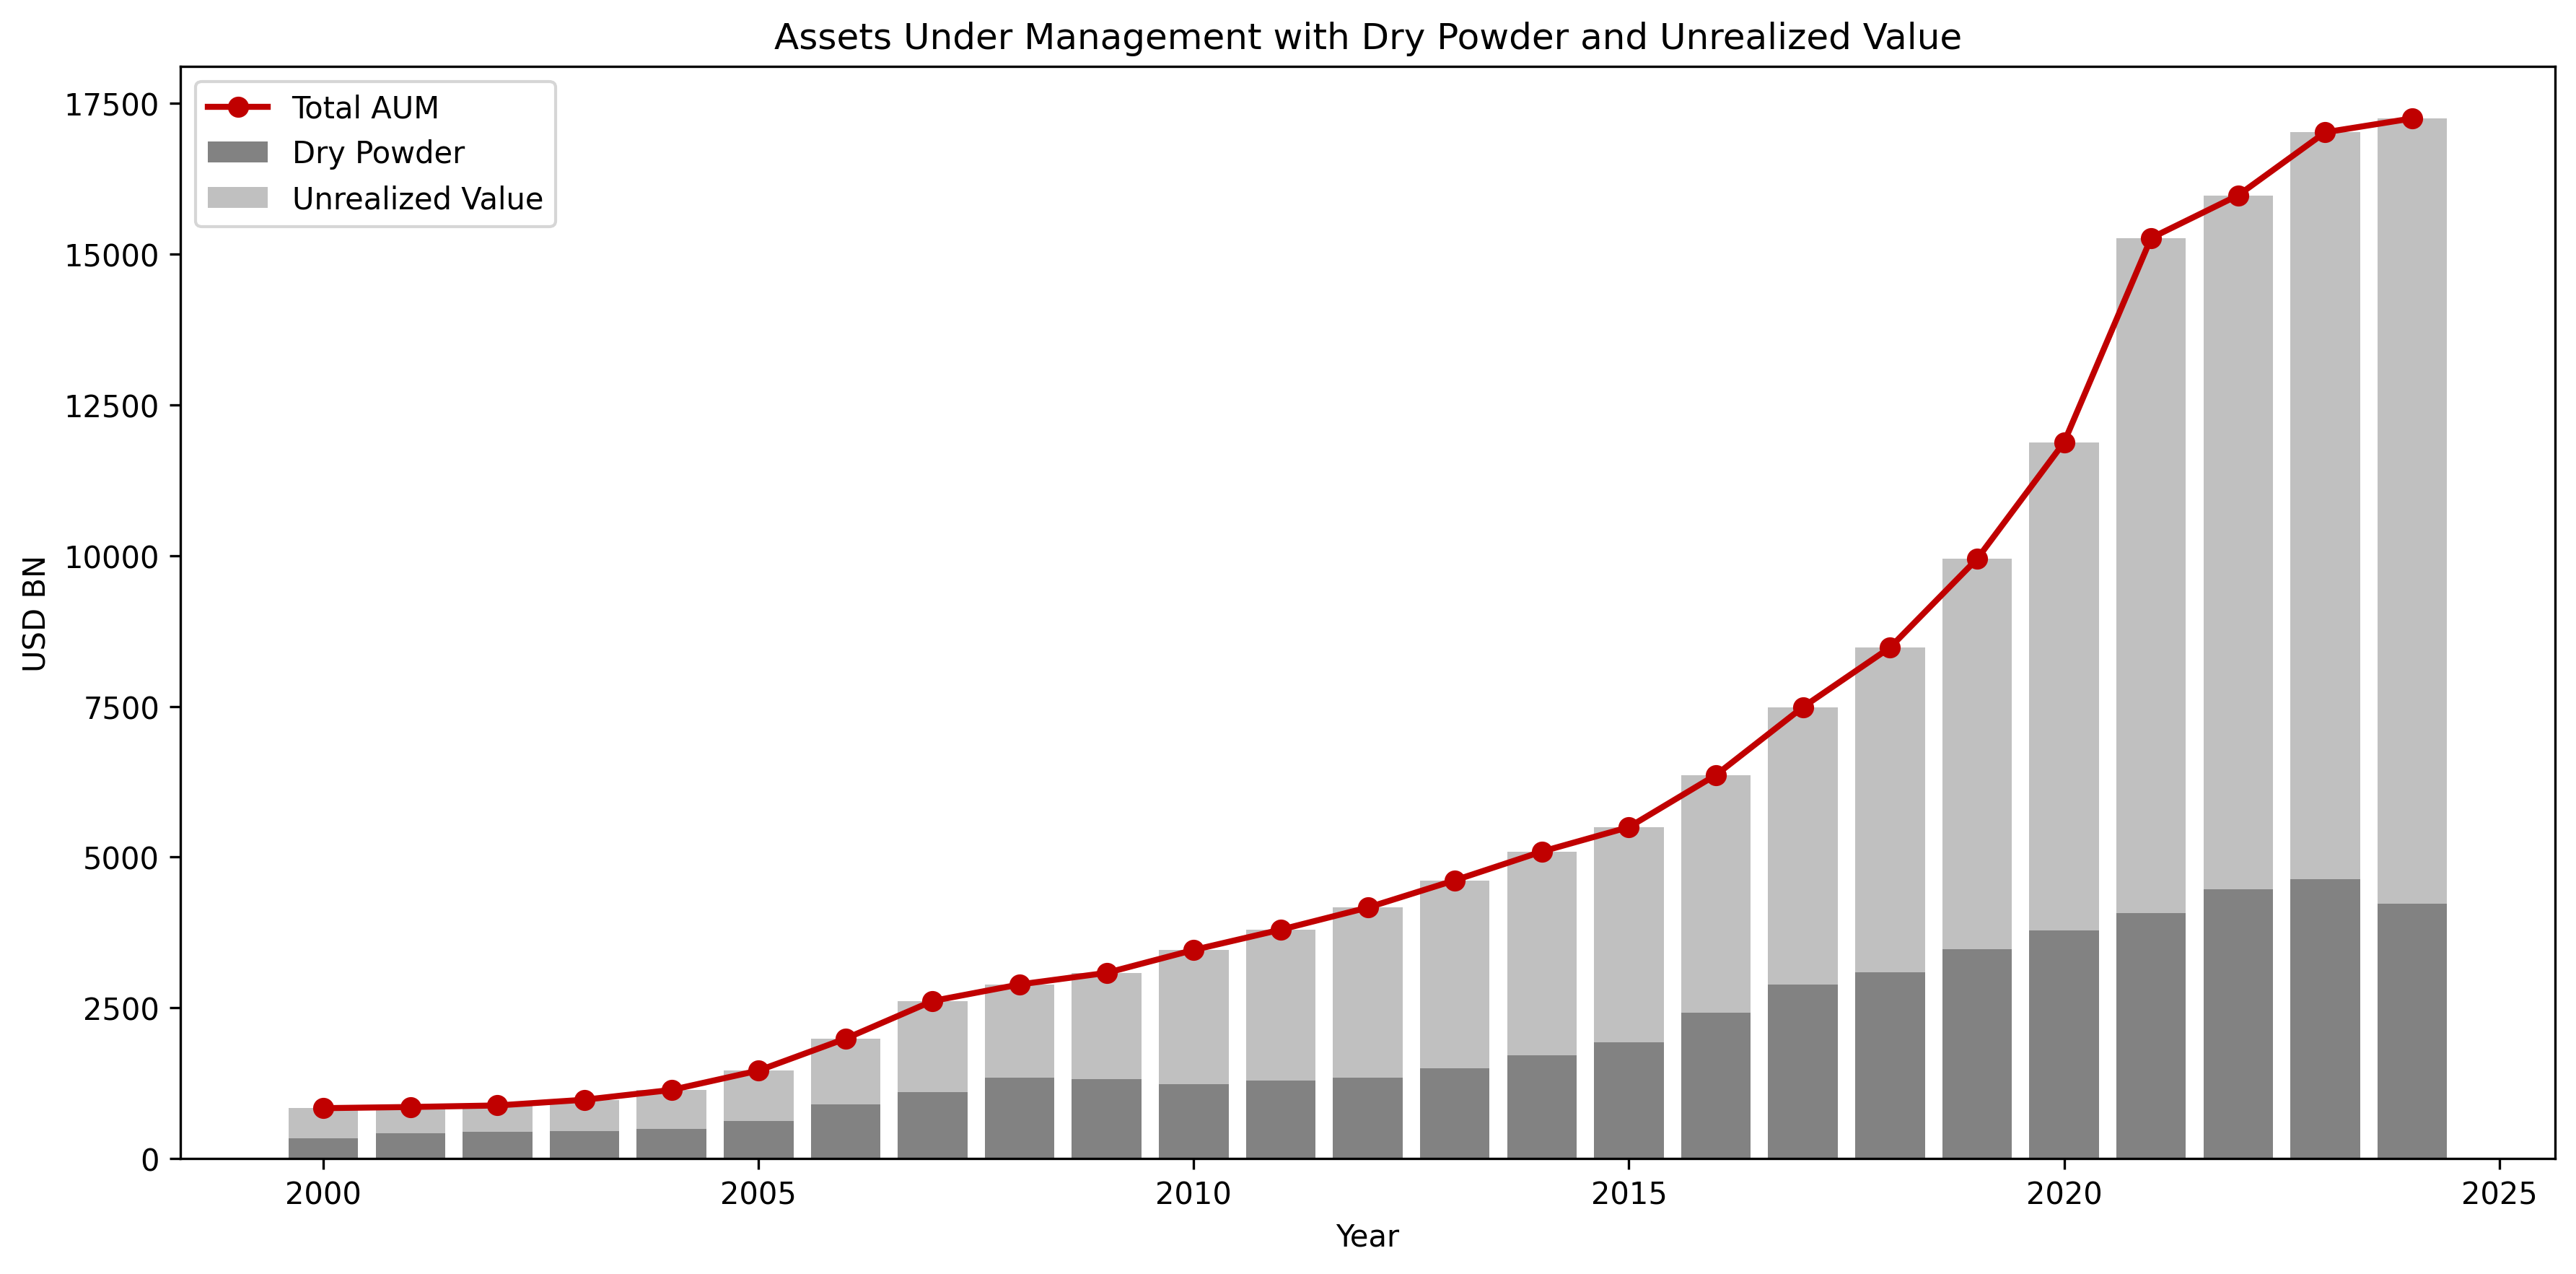
\includegraphics[width=\linewidth]{img/aum_drypowder_unrealized}
        \caption{PE assets under management, dry powder, and unrealized value.}
        \label{fig:aum_drypowder}
    \end{subfigure}
    \caption{Trends in private equity cash flows and capital. Data from Preqin.}
    \label{fig:pe_trends}
\end{figure}

In fact, unlike public equities, where investor beliefs can be inferred directly from market prices, private equity beliefs are not observable in real time.
Limited partners (LPs) form expectations about future distributions, exit values, and returns by interpreting a narrow set of signals: GP reports, due diligence materials, industry news, and historical cash flows.
GP communications often combine hard information with softer language that can influence perceptions, and it remains unclear whether LPs are consistently able to extract the predictive content of these narratives or if they are sometimes influenced by sentiment and bias.
Historical episodes illustrate the stakes: during the global financial crisis (2008-2009), many PE funds were slow to revise net asset values (NAVs), creating a disconnect between reported valuations and underlying fundamentals.
In contrast, during the COVID-19 shock, GPs initially issued cautious updates but quickly turned more optimistic as public markets recovered.
Both episodes suggest that GP communications can shape investor beliefs in ways not fully explained by fundamentals, with potential implications for capital allocation and risk perception (see Figure~\ref{fig:pe_vs_pm}).

\begin{figure}
    \centering
    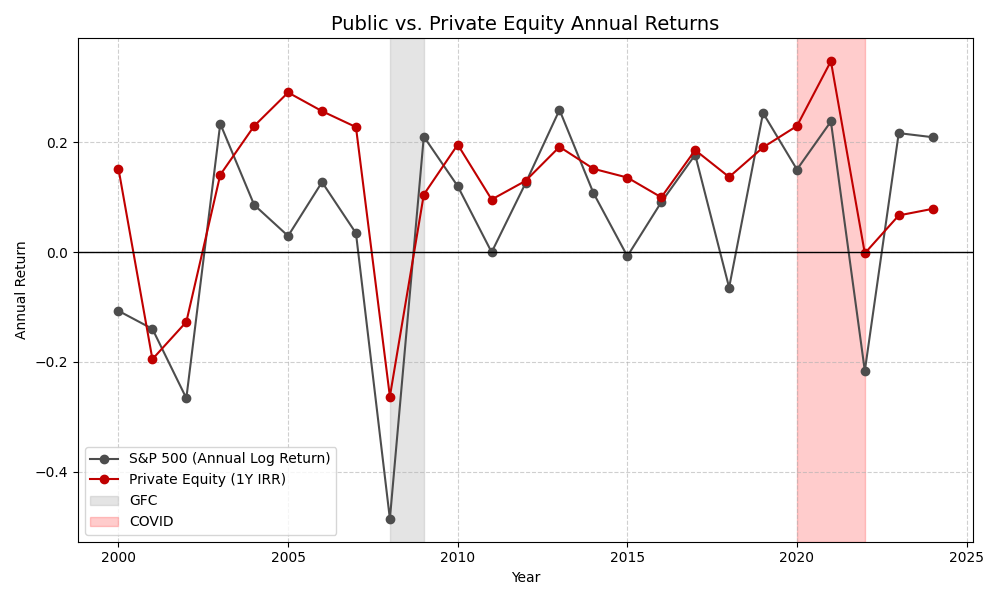
\includegraphics[width=0.8 \linewidth]{img/pe_vs_pm}
    \caption{Private equity returns (source: Preqin) are calculated using the NAV reported by GPs. Therefore, they tend to be much less elastic than market returns.}
    \label{fig:pe_vs_pm}
\end{figure}

Recent advances in natural language processing (NLP) and the emergence of large language models (LLMs) offer a new lens to examine these dynamics.
LLMs can process complex textual information and generate probabilistic forecasts based on contextual cues, mimicking or even surpassing human
interpretation.
In public markets, LLMs have already been shown to match human analysts performances when it comes to predict returns, infer sentiment, and identify risk exposures from unstructured data.
However, private markets present a more challenging environment: the data is scarcer, disclosures are less standardized, and outcomes are realized over long horizons.
The aim of this thesis is to introduce a methodology to use LLMs to process GPs report to extract information effectively and quantify the sentiment expressed by these documents.

\section{Literature Review}\label{sec:literature-review}

Classical models assume rational expectations, where investors form unbiased forecasts given available information.
Yet empirical evidence shows that beliefs often deviate systematically from fundamentals.
Behavioral models document patterns such as overreaction to recent performance, underreaction to fundamentals, and herding behavior~\citep{barberis2018behavioral}, observed in analyst forecasts, mutual fund flows, and investor reactions to earnings announcements.
In public markets, these biases are frequently linked to the use of heuristics when processing complex signals.

The starting point for this thesis is the literature is the work of~\cite{bybee2025ghost}.
\cite{bybee2025ghost} introduces a framework in which belief formation is shaped by language patterns.
Comparing human analyst reports and LLM-generated forecasts in response to news, he finds that both humans and models overweight recent returns, anchor on past price movements, and underweight fundamentals.
This suggests that beliefs can be modeled as processes influenced by the statistical patterns embedded in language rather than purely rational inference.

Private equity adds further complexity.
Unlike public equities, PE valuations are not continuously updated, and information flows are limited to periodic GP reports and occasional external assessments.
Recent work emphasizes how investor beliefs and biases shape asset prices, even in settings where fundamentals are difficult to observe.
For instance, \cite{ermakov2024believe} highlight the role of subjective beliefs in private equity valuation, showing that reported performance can diverge from underlying fundamentals depending on how narratives are interpreted.
Similarly, \cite{brown2022finding} study how institutional investors select asset managers, pointing to the importance of qualitative signals in decision-making.
Reported NAVs may be smoothed or manipulated, particularly around fundraising events or during market downturns~\citep{brown2008private}.
\cite{gupta2020valuing} show that when PE cash flows are decomposed into exposures to risk factors, most apparent outperformance disappears, and risk-adjusted returns are often negative.
This indicates that beliefs based solely on NAVs are likely distorted.
The scarcity and opacity of information in private markets amplify the role of narratives and subjective judgment, making them a natural extension of Bybee’s framework.

\subsection{LLMs in Finance}\label{sec:llms-in-finance}

The rapid development of large language models has opened new avenues for extracting predictive signals from unstructured financial data.
Early applications have focused on public markets, where extensive news, analyst reports, and earnings calls provide rich training grounds.
Studies show that LLMs can generate forecasts that incorporate complex qualitative information, often matching or exceeding traditional models in sentiment analysis and event prediction~\citep{ke2019machine, chen2023finbert}.
However, these applications rely on abundant and standardized textual data—conditions that do not hold in private markets.

\cite{fernandez2023limited} apply machine learning to textual disclosures in private placement memorandums.
They find that while investors often fail to use qualitative signals effectively, algorithms leveraging textual features achieve strong predictive power for fund performance.
Nuanced textual information, such as references to operational expertise, networks, or strategy, contains latent signals of skill that human investors often overlook.
This underscores the potential of AI-driven analysis in opaque markets and motivates the application of LLMs to belief formation in private equity.

\section{Research Question and Contributions}\label{sec:research-question-and-contributions}

Against this backdrop, the central research question of this thesis is:

\begin{quote}
    \emph{Are LLMs able to understand PE investment reports and form quantitative beliefs? How accurate are they?}
\end{quote}

To address this question, I leverage a dataset of over 20,000 PE investment reports from Preqin, enriched with cash flow data on capital calls and distributions.
The reports provide information on portfolio companies, market outlooks, and fund strategies in the unstructured format that LLMs are designed to process.
By  extracting belief measures directly from this text and comparing them to realized outcomes, I can test whether PE disclosures contain predictive
content and whether LLM-generated beliefs exhibit systematic biases.

This thesis makes three contributions:

\begin{enumerate}
    \item \textbf{Measurement of Beliefs:} I extend Bybee's methodology
    to quantify beliefs in private equity by applying LLMs to GP
    communications and extracting structured forecasts from unstructured
    text.
    \item \textbf{Implications for Asset Pricing and Allocation:} By linking
    text-derived beliefs to realized cash flows and factor-adjusted
    performance, I provide evidence on whether beliefs contain incremental
    information for forecasting PE outcomes.
    \item \textbf{Grounds for further research:} I provide ideas for further research.
\end{enumerate}